% ******** DO NOT EDIT ****************
\documentclass[10pt]{article}
% \usepackage{mathptmx}
\usepackage[letterpaper,margin=20mm]{geometry}
\usepackage{graphicx}
\usepackage{lmodern}
\renewcommand{\familydefault}{\sfdefault}
\pagestyle{empty}
\setlength{\parskip}{0.25\baselineskip}
\renewcommand{\title}[1]{{\noindent\large\bfseries#1\medskip\\}}
\renewcommand{\author}[2]{{\noindent #1 \medskip\\ \noindent \small #2 \medskip\\}}
% *************************************

\begin{document}

% ********** USER DEFINED *************

% Enter title here
\title{Phase Transitions in Homophilic Social Contagion}
\author{
% Enter author(s) here
Aníbal Olivera Morales\textsuperscript{1}, Jorge Fábrega Lacoa\textsuperscript{1}
}
{
% Enter affiliation(s) here
1. Centro de Investigación en Complejidad Social (CICS), Universidad del Desarrollo, Chile\\
}

% Enter abstract here. Please keep everything within one page.
Critical phenomena, particularly phase transitions where small parameter changes trigger massive cascades, are well documented in physical models. However, mapping criticality in meaning-bearing social systems remains a frontier challenge. While traditional models of collective behavior [1] and social contagion often assume either simplistic random topologies or homogeneous influence, empirical reality is driven by homophily—the tendency of similar individuals to cluster. In this work, we demonstrate that macro-level phase transitions in social adoption are an emergent property inextricably linked to these homophilic networks structures.

We address the scarcity of whole-network data in representative surveys by developing an imputation pipeline following [3]. By estimating homophily parameters from ego-centric data (GSS 2004) and imputing plausible network structures to large-scale attitudinal surveys (ATP 2016), we create empirical social topologies. On these networks, we simulate diffusion using a hybrid model: nodes adopt based on either Rational Choice (intrinsic utility) or Selective Social Influence. Our model extends classic threshold models [2] by explicitly treating social proximity as a weight for influence, allowing us to map the system's parameter space.

Using Intrinsic Utility Level (IUL) [1] as an external driving field and Maximum Social Proximity (MSP) as an analogue to thermodynamic temperature, our simulations map the parameter space of social contagion. MSP modulates the system's structural porosity: low MSP ``freezes'' the network into strict homophilic echo chambers, while high MSP ``melts'' these boundaries, allowing influence to flow more freely. We observe pronounced second-order phase transitions bounded by significant fluctuations (susceptibility) where social reinforcement abruptly overcomes local resistance (Figure 1). For initial regimes of low IUL, mass adoption emerges uniquely as a collective behavior that cannot be explained by examining individual interests alone, revealing contexts where society behaves analogous to complex matter. Crucially, comparing these empirical networks against degree-preserving Erdős-Rényi baselines via Generalized Additive Models (GAMs) reveals a systematic displacement of the critical boundary. Rather than merely enabling criticality, empirical clustering and homophily stretch and reshape the phase space, supporting massive contagion avalanches under less demanding combinations of temperature and external drive. Indeed, we find that randomizing the topography collapses this structural premium, reducing the overall odds of contagion by ~57\%. Ultimately, homophily acts as a structural catalyst that configures the critical regimes of social diffusion.

\begin{figure}[!h]
  \centering
  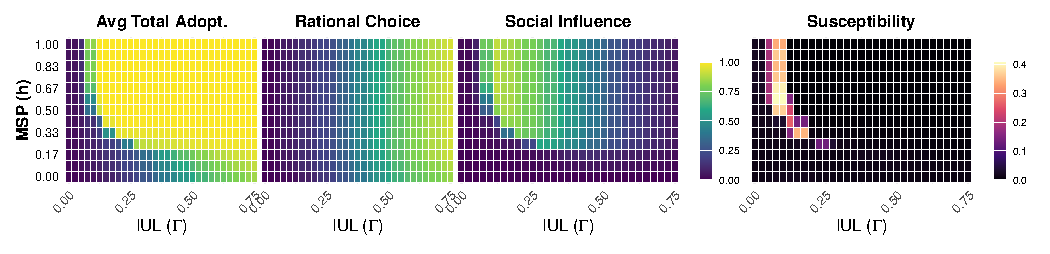
\includegraphics[width=1.0\textwidth]{figure.pdf}
  \vspace{-2mm}
  \caption{Criticality and the Phase Boundary in Social Contagion. Left to right: Average Total Adoption, Rational Choice Adoption, Social Influence Adoption, and Susceptibility. The empirical social topology exhibits a sharp second-order phase transition marked by a peak in susceptibility. Contagion avalanches (social influence) emerge within a narrow, highly sensitive critical space dictated by combinations of inherent utility (driving field) and social flexibility (temperature).}
\end{figure}

\bigskip
{\small
\noindent[1] Tur, E.M., Zeppini, P., \& Frenken, K. (2024). Diffusion in small worlds with homophily and social reinforcement. \textit{Social Networks}, 76, 12-21.\\
\noindent[2] Valente, T. W. (1996). Social network thresholds in the diffusion of innovations. \textit{Social Networks}, 18(1), 69-89.\\
\noindent[3] McPherson, M., \& Smith, J. A. (2019). Network effects in Blau space: Imputing social context from survey data. \textit{Socius}, 5, 2378023119865457.\\
\noindent[4] Granovetter, M. (1978). Threshold models of collective behavior. \textit{American Journal of Sociology}, 83(6), 1420–1443.
}

% *************************************
\end{document}
